\chapter{Matrix Decompositions}

\section{SVD}

We have seen that hermitian matrices are always diagonalizable. What about general rectangular matrices?
The following theorem shows that one can always find two matrix $\bold{U}$ and $\bold{V}$
so that the matrix $\bold{U}^H\bold{A}\bold{V}$ will be diagonal. This can be written as 
$\bold{U}^H\bold{A}\bold{V} = \bold{\Sigma }$ or equivalently, $\bold{A} = \bold{U}\bold{\Sigma }\bold{V}^H$.

\begin{figure}[htbp]
    \centering
    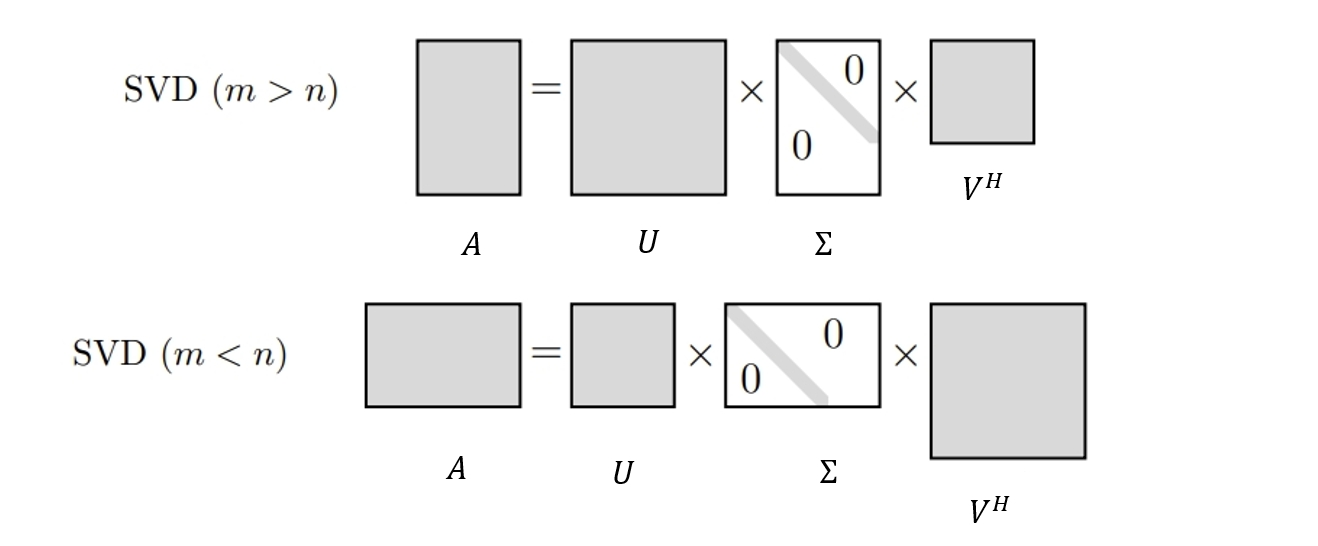
\includegraphics[width=0.6\textwidth]{figure/svd1.png}
    \caption{}
\end{figure}

\begin{remark}
    $\Sigma\in\C^{m\times n}$ is said to be diagonal if $\Sigma_{ij}=0$ for $i\neq j$.
    It has exactly $p=\min \{m,n\}$ diagonal entries and can be denoted by $\Sigma=\text{diag}\{d_1,...d_p\}$.
\end{remark}


\subsection{Singular value decomposition (SVD)}

\begin{proposition}{}{}
    For any matrix $\bold{A}\in \C^{m\times n}$, 
    $\bold{A}^H\bold{A}$ and $\bold{A}\bold{A}^H$ have non-negative eigenvalues.
\end{proposition}

\begin{proof}
    $\bold{A}^H\bold{A}$ and $\bold{A}\bold{A}^H$ are hermitian and positive semi-definite.
\end{proof}

\begin{proposition}{}{}
    For any matrix $\bold{A}\in \C^{m\times n}$, $r(\bold{A})=r(\bold{A}^H\bold{A})=r(\bold{A}\bold{A}^H)$.
\end{proposition}
\begin{proof}
    For $\bold{x}$, $\bold{Ax}=\bold{0}\Rightarrow \bold{A}^H\bold{Ax}=0$.
    For $\bold{x}$, $\bold{A}^H\bold{Ax}=\bold{0}\Rightarrow \bold{x}^H\bold{A}^H\bold{Ax}=\bold{0}\Rightarrow ||\bold{Ax}||_2^2=0\Rightarrow \bold{Ax}=\bold{0}$.
    Hence, $\text{dim(ker } \bold{A})=\text{dim(ker } \bold{A}^H\bold{A})$ and so $r(\bold{A})=r(\bold{A}^H\bold{A})$. 
    The result follows since $r(\bold{A}\bold{A}^H)=r(\bold{A}^H\bold{A})$.
\end{proof}

\begin{theorem}{}{}
    Let $\bold{A}\in \C^{m\times n}$ and denote $p=\min\{m,n\}$.
    Denote the rank of $\bold{A}$ by $r$ ($0\leqs r\leqs p$).
    Then there are unitary matrices $\bold{U}\in \C^{m\times m}$ and $\bold{V}\in \C^{n\times n}$
    and a real diagonal matrix $\Sigma =\text{diag} \{\sigma_1,...,\sigma_p\}\in \R^{m\times n}$ such that 
    \begin{align*}
        \bold{A}=\bold{U}\bold{\Sigma}\bold{V}^H
    \end{align*}
    and 
    \begin{align*}
        \sigma_1\geqs ...\geqs \sigma_r\geqs \sigma_{r+1}=...=\sigma_p=0,
    \end{align*}
    the matrix $\Sigma$ is uniquely determined by $\bold{A}$.
\end{theorem}

\noindent\textbf{Proof Strategy:} 
Assume $m>n$,
if $\bold{A}=\bold{U}\bold{\Sigma}\bold{V}^H$,
then 
\begin{align*}
    \bold{A}^H\bold{A}&=\bold{V}(\bold{\Sigma}^H\bold{\Sigma})\bold{V}^H\\
                        &=\bold{V}(\begin{bmatrix}
                            \sigma_{1} & & & & &\\
                            & \ddots & & & &\\
                            & & \sigma_{r} & & &\\
                            & & & & & \\
                          \end{bmatrix}\begin{bmatrix}
                            \sigma_{1} & & &\\
                            & \ddots & &\\
                            & & \sigma_{r} &\\
                            & & & \\
                            & & &
                          \end{bmatrix})\bold{V}^H & (\sigma_i^*=\sigma_i \text{ since }\sigma_i \in \R)\\
                        &=\bold{V}
                          \begin{bmatrix}
                            \sigma_{1}^2 & & &\\
                            & \ddots & &\\
                            & & \sigma_{r}^2 &\\
                            & & & \\
                          \end{bmatrix}\bold{V}^H
\end{align*}
Then we can let $\bold{V}$ be matrix containing the eigenvectors of $\bold{A}^H\bold{A}$
and $\bold{\Sigma}$ be matrix containing square roots of eigenvalues of $\bold{A}^H\bold{A}$.
After we have found both $\bold{V}$ and $\bold{\Sigma}$, rewrite the matrix equation as
\begin{align*}
    \bold{AV}=\bold{U\Sigma},
\end{align*}  
or in columns,
\begin{align*}
    \bold{A}\begin{pmatrix}
        \bold{v}_1&...&\bold{v}_r&\bold{v}_{r+1}&...&\bold{v}_n
    \end{pmatrix}
    = \begin{pmatrix}
        \bold{u}_1&...&\bold{u}_r&\bold{u}_{r+1}&...&\bold{u}_n
    \end{pmatrix}
    \begin{bmatrix}
        \sigma_{1} & & &\\
        & \ddots & &\\
        & & \sigma_{r} &\\
        & & & \\
        & & &
      \end{bmatrix}
\end{align*}
By comparing columns, we obtain
\begin{align*}
    \bold{X}\bold{v}_i=\left\{\begin{matrix}
        \sigma_i\bold{u}_i,&  1\leqs i\leqs r (\text{nonzero singular values})\\
        \bold{0},&  r<i\leqs d.
       \end{matrix}\right.
\end{align*}
This tells us how to find the matrix $\bold{U}: \bold{u}_i =\frac{1}{\sigma_i}\bold{A}\bold{v}_i$ for $1\leqs i\leqs r$.


\begin{proof}
    Let $\bold{C}=\bold{A}^H\bold{A}\in \C^{n\times n}$. Then $\bold{C}$ is square, hermitian, and positive semidefinite.
    Therefore, $\bold{C}=\bold{V}\Lambda\bold{V}^H$ for an unitary $\bold{V}\in \C^{n\times n}$
    and diagonal $\Lambda=\text{diag} \{\lambda_1,...\lambda_n\}\in \R^{n\times n}$ with $\lambda_1\geqs ...\geqs \lambda_r>0=\lambda_{r+1}=...=\lambda_n$.
    Let $\sigma_i=\sqrt{\lambda_i}$ and correspondingly form the matrix $\Sigma\in\R^{m\times n}$:
    \begin{align*}
        \bold{\Sigma} = \begin{pmatrix}
            \text{diag}(\sigma_1,...,\sigma_r) &\bold{O}_{r\times (n-r)}\\
            \bold{O}_{(m-r)\times r} &\bold{O}_{(m-r)\times (n-r)}
        \end{pmatrix}
    \end{align*}
    Define also
    \begin{align*}
        \bold{u}_i=\frac{1}{\sigma_i}\bold{A}\bold{v}_i\in\C^n, \text{ for each } 1\leqs i\leqs r.
    \end{align*}
    Then $\bold{u}_1,...,\bold{u}_r$ are orthonormal vectors. To see this,
    \begin{align*}
        \bold{u}_i^H\bold{u}_j &= (\frac{1}{\sigma_i} \bold{A}\bold{v}_i)^H (\frac{1}{\sigma_j}\bold{A}\bold{v}_j) = \frac{1}{\sigma_i\sigma_j} \bold{v}_i^H\bold{A}^H\bold{A}\bold{v}_j\\
        &= \frac{1}{\sigma_i\sigma_j} \bold{v}_i^H(\lambda_jv)
    \end{align*}
\end{proof}

\subsection{Geometric interpretation of SVD}

\subsection{Applications of Singular-Value Decomposition}

\section{Reference}

\begin{itemize}
    \item \href{http://users.ece.northwestern.edu/~mya671/files/Matrix_YM_.pdf}{Matrix Decomposition}
    \item \href{https://math.berkeley.edu/~hutching/teach/54-2017/svd-notes.pdf}{SVD notes}
    \item \href{https://www.sjsu.edu/faculty/guangliang.chen/Math253S20.html}{Mathematical Methods for Data Visualization}
    \item \href{https://kuidu.github.io/nla/nla02.pdf}{SVD notes XMUT}
    \item \href{https://people.cas.uab.edu/~mosya/teaching/660new3.pdf}{Singular Value Decomposition}
    \item \href{https://www2.math.uconn.edu/~leykekhman/courses/MATH3795/Lectures/Lecture_9_Linear_least_squares_SVD.pdf}{least squares svd}
    \item \href{https://math.ucsd.edu/sites/math.ucsd.edu/files/undergrad/honors-program/honors-theses/2017-2018/Zecheng_Kuang_Honors_Thesis.pdf}{svd application}
\end{itemize}